%
% 1-gamma.tex -- Abschnitt über die Gamma-funktion
%
% (c) 2021 Prof Dr Andreas Müller, OST Ostschweizer Fachhochschule
%
\section{Die Gamma-Funktion
\label{buch:rekursion:section:gamma}}
\rhead{Gamma-Funktion}
Die Fakultät $x!$ kann rekursiv durch 
\[
	x! = x\cdot (x-1)! \qquad\text{und}\qquad 0!=1
\]
für alle natürlichen Zahlen $x\in\mathbb{N}$ definiert werden.
Äquivalent damit ist eine Funktion 
\begin{equation}
\Gamma(x+1) = x\Gamma(x)
\qquad\text{und}\qquad 
\Gamma(1)=1.
\label{buch:rekursion:eqn:gammadef}
\end{equation}
Kann man eine reelle oder komplexe Funktion finden, die die
Funktionalgleichung~\eqref{buch:rekursion:eqn:gammadef}
\index{Gamma-Funktion!Funktionalgleichung}%
\index{Funktionalgleichung der Gamma-Funktion}%
erfüllt und damit die Fakultät auf beliebige Argumente ausdehnt?

%
% Definition als Grenzwert
%
\subsection{Definition als Grenzwert}
Die Fakultät $n!$ ist ein Produkt von $n$ Faktoren, es ist daher
natürlich zu versuchen, auch $x!$ als ein Produkt zu schreiben.
Allerdings kann es nicht möglich sein, dies mit einer endlichen
Anzahl von Faktoren zu machen, denn wenn $x$ grösser wird, muss auch
die Zahl der Faktoren grösser werden.
Mit jedem zusätzlichen Faktor ist ein Sprung der Werte zu erwarten.
Wir erwarten daher entweder ein unendliches Produkt oder einen
Ausdreck, bei dem die ``Anzahl'' $x$ der Faktoren im Exponenten
steht.
In diesem Abschnitt soll zunächst eine solcher Ausdruck gefunden
werden.
Dieser ist jedoch für die numerische Berechnung absolut ungeeignet,
so dass er später in ein unendliches Produkt umgeformt werden muss.

%
% Fakultät als Bruch
%
\subsubsection{Fakultät als Bruch}
Euler hat das Problem, die Fakultät auf beliebige reelle oder komplexe
Zahlen auszudehnen, wie folgt angepackt.
Zunächst hat er bemerkt, dass für ganzzahlige $x$ und natürliche $n$
\begin{align}
x! 
&=
1\cdot 2\cdot 3\cdot\ldots\cdot x
\notag
\\
&=
\frac{
1\cdot 2\cdot 3\cdot\ldots\cdot x\cdot (x+1) (x+2)\cdots(x+n)
}{
(x+1)(x+2)\cdots(x+n)
}
\notag
\\
&=
\frac{
1\cdot 2\cdot\ldots\cdot n\cdot(n+1)\cdot(n+2)\cdots(n+x)
}{
(x+1)(x+2)\cdots(x+n)
}
\notag
\\
&=
\frac{n! \cdot (n+1)(n+1)\cdots(n+x)}{(x+1)(x+2)\cdots(x+n)}
\label{buch:rekursion:gamma:eqn:fakultaet}
\end{align}
gilt.
Der Plan ist, dies so umzuformen, dass man für $x$ eine beliebige
komplexe Zahl einsetzen kann.

%
% Pochhammer-Symbol
%
\subsubsection{Pochhammer-Symbol}
Die spezielle Form des Nenners und des zweiten Faktors im Zähler
von \eqref{buch:rekursion:gamma:eqn:fakultaet}
rechtfertigt die folgende Definition.

\begin{definition}[Pochhammer]
Für $a\in\mathbb{C}$ und $n\in\mathbb{N}$ heisst das Produkt
\[
(a)_n = a\cdot(a+1)\cdot(a+2)\cdots(a+n-1)
\]
das Pochhammer-Symbol oder die verschobene Fakultät.
\index{Pochhammer-Symbol}
\end{definition}

Die verschobene Fakultät $(a)_n$ hat also genau $n$ Faktoren, deren
erster $1$ ist.
Die gewöhnliche Fakultät hat $n$ Faktoren, deren erster $1$ ist, also
ist $n! = (1)_n$.

Der Ausdruck \eqref{buch:rekursion:gamma:eqn:fakultaet}
für $x!$ wird unter Verwendung des Pochhammer-Symbols zu
\begin{equation}
x! = \frac{n! (n+1)_x}{(x+1)_n}.
\label{buch:rekursion:gamma:eqn:produkt2}
\end{equation}
Leider ist dieser Ausdruck ebenfalls nicht auf beliebige $x$
verallgemeinerungsfähig, denn $(n)_x$ ist nur natürliche $x$ definiert.
Der Faktor $(n+1)_x$ enthält $x$ Faktoren beginnend bei $n$.
Für grosses $n$ sind diese Faktoren nahe beeinander, man sollte also
$(n+1)_x$ durch $n^x$ approximieren können.
Wir erweitern daher \eqref{buch:rekursion:gamma:eqn:produkt2} mit $n^x$
und erhalten
\begin{equation}
x!
=
\frac{n!\,n^x}{(x+1)_n}\cdot
\frac{(n+1)_x}{n^x}.
\label{buch:rekursion:gamma:eqn:produkt3}
\end{equation}
Der erste Faktor in diesem Ausdruck enthält jetzt nur noch Dinge,
die für beliebige $x\in\mathbb{C}$ definiert sind.

%
% Grenwertdefinition
%
\subsubsection{Grenzwertdefinition}
Der zweite Bruch in \eqref{buch:rekursion:gamma:eqn:produkt3}
besteht aus Termen, die zwar nur für natürliches $x$ definiert sind,
wir vermuten aber, dass er für grosses $n$ gegen $1$ konvergiert.
Tatsächlich gilt
\[
\lim_{n\to\infty}
\frac{(n+1)_x}{n^x}
=
\lim_{n\to\infty}
\underbrace{\frac{n+1}{n}}_{\displaystyle\to 1}
\cdot
\underbrace{\frac{n+2}{n}}_{\displaystyle\to 1}
\cdot\ldots\cdot
\underbrace{\frac{n+x}{n}}_{\displaystyle\to 1}
=
1,
\]
da  $(n+x)/n=1+x/n\to 1$ für grosses $n$.
Dies würde die folgende Definition rechtfertigen.

\begin{definition}
\label{buch:rekursion:gamma:def:definition}
Die Gamma-Funktion $\Gamma(x)$ einer Zahl
$x\in\mathbb{C}\setminus\{0,-1,-2,-3,\dots\}$ ist der Grenzwert
\[
\Gamma(x) = \lim_{n\to\infty} \frac{n!\,n^{x-1}}{(x)_n}.
\] 
\index{Grenzwertdefinition der Gamma-Funktion}%
\index{Gamma-Funktion!Grenzwertdefinition}%
\end{definition}

%
% Rekursionsgleichung für Gamma(x)
%
\subsubsection{Rekursionsgleichung für $\Gamma(x)$}
Es ist aus der Herleitung klar, dass $\Gamma(n)=(n-1)!$ sein muss.
Wir sollten dies aber auch direkt aus der
Definition~\ref{buch:rekursion:gamma:def:definition} ableiten
können.
Dazu müssen wir nur überprüfen, ob $\Gamma(1)=0!=1$ ist und ob
die Rekursionsformel $\Gamma(n)=n\Gamma(n-1)$ gilt.

Den Wert $\Gamma(1)$ kann man direkt berechnen:
\[
\Gamma(1)
=
\lim_{n\to\infty} \frac{n!}{(1)_n}
=
\lim_{n\to\infty} \frac{n!}{n!}
=
1
\]
wegen $(1)_n=n!$.

Für die Rekursionsformel muss man den Grenzwert für $x$ und $x+1$
miteinander vergleichen.
Aus dem Term $(x+1)_n$ im Nenner muss man einen Term $(x)_n$ machen,
dies ist möglich, indem man mit $x$ erweitert:
\begin{align*}
\Gamma(x+1)
&=
\lim_{n\to\infty}\frac{n!\,n^x}{(x+1)_n}
=
x\lim_{n\to\infty}\frac{n!\,n^x}{x(x+1)_n}
=
x\lim_{n\to\infty}\frac{n!\,n^x}{(x)_{n+1}}.
\intertext{Wir müssen jetzt nur noch zeigen, dass der Grenzwert
auf der rechten Seite gegen $\Gamma(x)$ konvergiert,
in dessen Definition aber die Potenz $n^{x-1}$ vorkommt.
Wir müssen also einen Faktor $n$ los werden und gleichzeitig
aus $n$ überall $n+1$ machen, damit der Nenner wieder passt.
Dabei wird}
\Gamma(x+1)
&=
x\lim_{n\to\infty}
\frac{(n+1)!n^{x-1}}{(x)_{n+1}}
\cdot
\underbrace{\frac{n}{n+1}}_{\displaystyle\to 1}
\\
&=
x\lim_{n\to\infty}
\underbrace{\frac{(n+1)!(n+1)^{x-1}}{(x)_{n+1}}}_{\displaystyle\to\Gamma(x)}
\cdot
\frac{n^{x-1}}{(n+1)^{x-1}}
\\
&=
x
\Gamma(x)
\lim_{n\to\infty} \biggl(\frac{n}{n+1}\biggr)^{x-1}
=
x\Gamma(x),
\end{align*}
Weil $n/(n+1)\to 1$ ist und die Funktion $z\mapsto z^{x-1}$ für alle
nach der Definition zulässigen Werte von $x$ eine stetige Funktion ist.

%
% Gamma-Funktion und Pochhammer-Symbol
%
\subsubsection{Gamma-Funktion und Pochhammer-Symbol}
Durch Iteration der Rekursionsformel für $\Gamma(x)$ folgt jetzt
\begin{align*}
\Gamma(x+n)
&=
(x+n-1) \Gamma(x+n-1)
\\
&=
(x+n-1)(x+n-2)\Gamma(x+n-2)
\\
&=
\underbrace{
(x+n-1)(x+n-2)\cdots(x-1)(x)
}_{\text{$n$ Faktoren}} \Gamma(x)
\\
&=(x)_n \Gamma(x).
\end{align*}
Damit folgt

\begin{satz}
\index{Satz!Pochhammer-Symbol@Pochhammer-Symbol und $\Gamma(x)$}%
\label{buch:rekursion:gamma:satz:gamma-pochhammer}
Die Rekursionsformel für die Gamma-Funktion kann geschrieben werden als
\[
\Gamma(x+n) = (x)_n \Gamma(x).
\]
Das Pochhammer-Symbol $(x)_n$ ist für alle natürlichen $n$ gegeben durch
\[
(x)_n = \frac{\Gamma(x+n)}{\Gamma(x)}.
\]
\end{satz}

%
% Numerische Unzulänglichkeit der Grenzwertdefinition
%
\subsubsection{Numerische Unzulänglichkeiten der Grenzwertdefinition}
\begin{table}
\centering
%\renewcommand{\arraystretch}{1.1}
\begin{tabular}{|>{$}c<{$}|>{$}r<{$}|>{$}l<{$}|>{$}l<{$}|}
\hline
\log_{10} n&           n&n!n^{x-1}/(x)_n\mathstrut     &       \text{Fehler%
\vrule height12pt depth6pt width0pt} \\
\hline
\text{\vrule height12pt depth0pt width0pt} 
          1&          10&1.\underline{7}947392559855804&0.0222854050800643\\
          2&         100&1.\underline{77}46707942830697&0.0022169433775536\\
          3&        1000&1.\underline{772}6754214755178&0.0002215705700017\\
          4&       10000&1.\underline{7724}760067171375&0.0000221558116213\\
          5&      100000&1.\underline{77245}60664742375&0.0000022155687214\\
          6&     1000000&1.\underline{77245}40724623101&0.0000002215567940\\
          7&    10000000&1.\underline{7724538}730613721&0.0000000221558560\\
          8&   100000000&1.\underline{77245385}31233258&0.0000000022178097\\
          9&  1000000000&1.\underline{77245385}11320680&0.0000000002265519\\
         10& 10000000000&1.\underline{772453850}9261316&0.0000000000206155\\
         11&100000000000&1.\underline{77245385}14549788&0.0000000005494627\\
           &      \infty&1.\underline{7724538509055161}&
\text{\vrule height12pt depth6pt width0pt} \\
\hline
\end{tabular}
\caption{Numerische Berechnung mit der Grenzwertdefinition
und rekursiver Berechnung von $n!/(x)_n$ mit Hilfe der Folge
\eqref{buch:rekursion:gamma:pnfolge}.
Die Konvergenz ist sehr langsam, die Anzahl korrekter Stellen
wächst logarithmisch mit $n$.
\label{buch:rekursion:gamma:produktberechnung}}
\end{table}
Die Grenzwertdefinition~\ref{buch:rekursion:gamma:def:definition}
ist zwar zweifellos richtig, kann aber nicht für die numerische 
Berechnung der Gamma-Funktion verwendet werden.
Die Existenz des Grenzwertes verwendet, dass $x\ll n$ sein muss,
damit $(n+x)/n$ gegenüber $1$ vernachlässigt werden kann.
Die Grenzwertdefinition beginnt also erst, vernünftige Approximationen
von $\Gamma(x)$ zu geben, wenn $n$ viel grösser also $x$ ist.
Andererseits wächst $n!$ sehr schnell an, schon für $n=171$ ist
das Resultat grösser als was der \texttt{double}-Datentyp fassen kann.
Dies ist aber viel zu kleine, um gute Approximationen auch für kleine
Werte von $x$ zu geben.
So findet man zum Beispiel für $x=\frac12$ und $n=170$ mit Octave
\[
\frac{n!\,n^{x-1}}{(x)_n}
=
\frac{170!}{\sqrt{170}\cdot \frac12\cdot\frac32\cdot\ldots\cdot\frac{339}{2}}
=
\frac{7.2574\cdot10^{307}}{13.308\cdot 3.1381\cdot10^{305}}
=
1.7738.
\]
Andererseits werden wir später sehen, dass 
\[
\Gamma({\textstyle\frac12})
=
\sqrt{\pi}
=
1.772453850905516
\]
ist.
Die Approximation mit Hilfe der Grenzwertdefinition kann also
grundsätzlich nicht mehr als zwei korrekte Nachkommastellen liefern.

Den Quotienten $n!/(x)_n$ kann man mit Hilfe der Rekursionsformel
\begin{equation}
p_n = p_{n-1}\cdot \frac{n}{x+n-1},\qquad
p_0 = 0
\label{buch:rekursion:gamma:pnfolge}
\end{equation}
etwas effizienter berechnen. 
Insbesondere umgeht man damit das Problem, dass $n!$ den Wertebereich 
des \texttt{double} Datentyps sprengt.
Der Wert der Gamma-Funktion kann dann durch $p_nn^{x-1}$ approximiert
werden.
Die Tabelle~\ref{buch:rekursion:gamma:produktberechnung} fasst die
Resultate zusammen und zeigt, dass die Konvergenz logarithmisch ist:
die Anzahl korrekter Nachkommastellen ist $\log_{10}n$.

%
% Produktformel
%
\subsection{Produktformel}
Ein möglicher Ausweg aus den numerischen Schwierigkeiten mit der
Grenzwertdefinition ist, den schnell wachsenden Faktor $n!$
in den Zähler zu bringen, so dass er der Konvergenz etwas nachhilft.
Wir berechnen daher den Kehrwert $1/\Gamma(x)$.

\begin{satz}
\index{Satz!Produktformel@Produktformel für $\Gamma(x)$}%
\label{buch:rekursion:gamma:satz:produktformel}
Der Kehrwert der Gamma-Funktion kann geschrieben werden als
\begin{equation}
\frac{1}{\Gamma(x)}
=
xe^{\gamma x}
\prod_{k=1}^\infty
\biggl(1+\frac{x}k\biggr)\,e^{-\frac{x}{k}},
\label{buch:rekursion:gamma:eqn:produktformel}
\index{Gamma-Funktion!Produktformel}%
\end{equation}
wobei $\gamma$ die Euler-Mascheronische Konstante
\index{Euler-Mascheronische Konstante}%
\[
\gamma
=
\lim_{n\to\infty}
\biggl(\sum_{k=1}^n\frac{1}{k}-\log n\biggr)
\]
ist.
\index{Gamma-Funktion!Produktformel}%
\index{Produktformel für die Gamma-Funkion}%
\end{satz}

\begin{proof}[Beweis]
Es sind zwei Dinge nachzuprüfen.
Zunächst muss nachgewiesen werden, dass das unendliche Produkt 
überhaupt konvergiert.
Wenn das gesichert ist, muss noch gezeigt werden, dass der Grenzwert
tatsächlich $1/\Gamma(x)$ ist.

Für die Konvergenz beachtet man, dass die Faktoren des Produkts 
die Form
\begin{align*}
\biggl(1+\frac{x}n\biggr)e^{-\frac{x}{n}}
&=
\biggl(1+\frac{x}n\biggr)
\biggl(1-\frac{x}{n}+\frac{x^2}{2n^2}-\frac{x^3}{3!n^3}+\dots\biggr)
\\
&=
1-\frac{x^2}{n^2} + 
\biggl(1+\frac{x}n\biggr)
\biggl(\frac{x^2}{2n^2}-\dots\biggr)
\\
&=
1-\frac{x^2}{n^2} + \frac{x^2}{2n^2} + O\bigl((\textstyle\frac{x}{n})^2\bigr)
\\
&=
1-\frac{x^2}{2n^2} + O\bigl((\textstyle\frac{x}{n})^3\bigr)
\end{align*}
haben.
Da die Reihe 
\[
\sum_{n=1}^\infty \frac{x^2}{n^2}
\]
konvergent ist, konvergiert auch das Produkt.
% XXX wir brauchen irgendwo das Konvergenzkriterium für ein Produkt

Um die Übereinstimmung der Produktformel mit $1/\Gamma(x)$ zu zeigen,
berechnen wir
\begin{align*}
\frac{1}{\Gamma(x)}
&=
\lim_{n\to\infty} 
\frac{(x)_n}{n!\,n^{x-1}}
=
\lim_{n\to\infty} 
\frac{x(x+1)(x+2)\cdots(x+n-1)}{1\cdot 2\cdot3\cdots (n-1)\cdot n\cdot n^{x-1}}
\\
&=
x
\lim_{n\to\infty} 
\frac{x+1}{1}
\cdot
\frac{x+2}{2}
\cdots
\frac{x+n-1}{n-1}
\cdot
n^{-x}
\\
&=
x
\lim_{n\to\infty}
\biggl(1+\frac{x}{1}\biggr)
\cdot
\biggl(1+\frac{x}{2}\biggr)
\cdots
\biggl(1+\frac{x}{n-1}\biggr)
\cdot
e^{-x\log n}
\\
&=
x
\prod_{k=1}^{n-1}
\biggl(1+\frac{x}{k}\biggr)
e^{-\frac{x}{k}}
e^{\frac{x}{k}}
e^{-x\log n}
\\
&=
x
\biggl(
\lim_{n\to\infty}
\prod_{k=1}^{n-1}
\biggl(1+\frac{x}{k}\biggr)
e^{-\frac{x}{k}}
\biggr)
\cdot
\biggl(
\lim_{n\to\infty}
e^{x\bigl(\sum_{k=1}^{n-1}\frac{1}{k} - \log n\bigr)}
\biggr)
\end{align*}
Der Klammerausdruck im Exponent des letzten Faktors auf der rechten Seite
konvergiert nach Definition der Euler-Mascheronischen Konstanten gegen
$\gamma$, somit folgt 
\[
\frac{1}{\Gamma(x)}
=
xe^{\gamma x}\prod_{k=1}^\infty \biggl(1+\frac{x}{k}\biggr)e^{-\frac{x}{k}},
\]
wie behauptet.
Damit ist Satz~\ref{buch:rekursion:gamma:satz:produktformel}
vollständig bewiesen.
\end{proof}

\begin{table}
\centering
\begin{tabular}{|>{$}c<{$}|>{$}r<{$}|>{$}c<{$}|>{$}c<{$}|}
\hline
k & n &  \Gamma(\frac12,n) & \Gamma(\frac12) - \Gamma(\frac12,n)%
\text{\vrule height12pt depth6pt width0pt} \\
\hline
\text{\vrule height12pt depth0pt width0pt} 
     1&     10& 1.\underline{7}518166478& -0.0206372031 \\
     2&    100& 1.\underline{77}02543372& -0.0021995137 \\
     3&   1000& 1.\underline{772}2324556& -0.0002213953 \\
     4&  10000& 1.\underline{7724}316968& -0.0000221541 \\
     5& 100000& 1.\underline{77245}16354& -0.0000022156 \\
     6&1000000& 1.\underline{772453}6293& -0.0000002216 \\
\infty&       & 1.\underline{7724538509}&
\text{\vrule height12pt depth6pt width0pt} \\
\hline
\end{tabular}
\caption{Werte $\Gamma(\frac12,n)$ von $\Gamma(\frac12)$ berechnet mit
$n=10^k$ Faktoren der
Produktformel~\eqref{buch:rekursion:gamma:eqn:produktformel}
und der zugehörige Fehler.
Die korrekten Nachkommastellen sind unterstrichen.
Die Konvergenz ist genau gleich langsam wie in der Berechnung mit
Hilfe der Grenzwert-Definition in
Tabelle~\ref{buch:rekursion:gamma:produktberechnung}.
\label{buch:rekursion:gamma:gammatabelle}}
\end{table}

Um zu zeigen, dass die Produktform tatsächlich besser geeignet ist,
sind in der Tabelle~\ref{buch:rekursion:gamma:gammatabelle}
die Resultate der numerischen Rechnung  bis $n=1000000$ zusammengestellt.
Die Produktformel kann gute Werte von $\Gamma(x)$ auch für derart grosse
Werte von $n$ problemlos berechnen.

Der Fehler der numersichen Approximation ist von der Grössenordnung
$O(1/n)$ wie das auf Grund des verwendeten Konvergenzkriteriums
zu erwarten war.
Die Anzahl zu berücksichtigender Terme wächst daher exponentiall
mit der Anzahl gewünschter Stellen an, was für praktische Zwecke
zu langsam ist.
Für die numersiche Berechnung der Gamma-Funktion ist die Produktformel
daher im Allgemeinen nicht geeignet.

%
% Integralformel für die Gamma-Funktion
%
\subsection{Integralformel für die Gamma-Funktion}
Euler hat die folgende Integraldefinition der Gamma-Funktion gegeben.

\begin{definition}
\label{buch:rekursion:def:gamma}
Die Gamma-Funktion ist die Funktion 
\begin{equation}
\Gamma
\colon
\{z\in\mathbb{C} \mid \operatorname{Re}z>0\}
\to \mathbb{C}
:
z
\mapsto
\Gamma(z) = \int_0^\infty t^{z-1}e^{-t}\,dt
\label{buch:rekursion:eqn:gammaintegral}
\end{equation}
\index{Gamma-Funktion!Integraldefinition}%
\index{Integraldefinition der Gamma-Funktion}%
\end{definition}

Man beachte, dass das Integral für $x=0$ nicht definiert ist, eine
Potenzreihenentwicklung um einen Punkt $x_0$ auf der positiven reellen
Achse kann also höchstens den Konvergenzradius $\varrho=|x_0|$ haben.

Die Definition~\ref{buch:rekursion:def:gamma} wird erst später in
\eqref{buch:rekursion:gamma:integralbeweis} auf
Seite~\pageref{buch:rekursion:gamma:integralbeweis} gegeben.
Im Folgenden wird zunächst verifiziert, dass die Integraldarstellung
die richtigen Werte für natürliche Argumente hat, es wird aber auch
gezeigt, dass dies nicht ausreicht um zu schliessen, dass die
Integralformel mit der früher definierten Gamma-Funktion übereinstimmt.

%
% Funktionalgleichung für die Integraldefinition
%
\subsubsection{Funktionalgleichung für die Integraldefinition}
Tatsächlich ist es einfach nachzuprüfen, dass die Funktionalgleichung
der Gamma-Funktion auch für die Definition~\ref{buch:rekursion:def:gamma}
Korrekt ist. 
Dazu ist zunächgst nachzurechnen, dass mindestens ein Wert der neuen 
Definition übereinstimmt mit der alten Definnition, zum Beispiel der
Wert
\[
\Gamma(1)
=
\int_0^\infty t^{1-1}e^{-t}\,dt
=
\biggl[ -e^{-t} \biggr]_0^\infty
=
1.
\]
Ausserdem muss die Funktionalgleichung erfüllt sein, also
\begin{align*}
\Gamma(z)
&=
\int_0^\infty
\underbrace{t^{z-1}}_{\displaystyle\uparrow}
\underbrace{e^{-t}}_{\displaystyle\downarrow}
\,dt
=
\underbrace{\biggl[
\frac{1}{z} t^z e^{-t}
\biggr]_0^\infty}_{\displaystyle=0}
+
\frac{1}{z}
\int_0^\infty
t^z e^{-t}
\,dt
=
\frac{1}{z}\Gamma(z+1)
\\
\Rightarrow\qquad
z\Gamma(z)&=\Gamma(z+1).
\end{align*}
Dies beweist aber nur, dass die beiden Definitionen für positiv
ganzzahlige Argumente übereinstimmen.
Der folgende Abschnitt macht deutlich, dass es sehr viele Funktionen gibt,
die ebenfalls die Funktionalgleichung erfüllen.
Eine vollständige Rechtfertigung für diese Definition wird später
in Abschnitt~\ref{buch:rekursion:gamma:subsection:integralbeweis}
in Formel~\eqref{buch:rekursion:gamma:integralbeweis}
auf Seite~\pageref{buch:rekursion:gamma:integralbeweis}
gegeben.

\begin{figure}
\centering
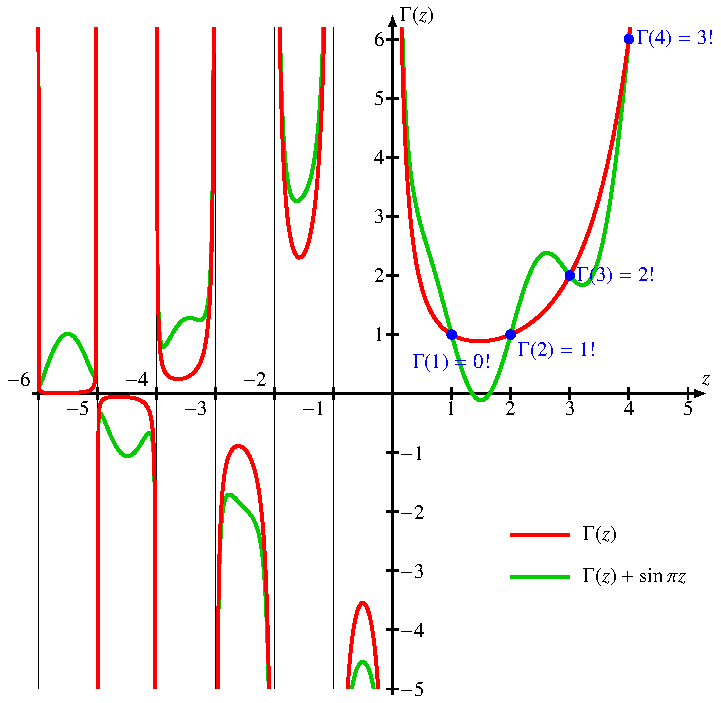
\includegraphics{chapters/040-rekursion/images/gammaplot.pdf}
\caption{Graph der Gamma-Funktion $z\mapsto\Gamma(z)$ und der alternativen
Funktion $\Gamma(z)+\sin(\pi z)$, die für ganzzahlige Argumente ebenfalls
die Werte der Fakultät annimmt.
\label{buch:rekursion:fig:gamma}}
\end{figure}

%
% Der Wert Gamma(1/2)
%
\subsubsection{Der Wert $\Gamma(\frac12)$}
Die Integraldarstellung kann dazu verwendet werden, $\Gamma(\frac12)$ 
zu berechnen.
\index{Gamma-Funktion!WertGamma12@Wert von $\Gamma(\frac12)$}%
\index{G(1/2)@$\Gamma(\frac12)$}%
Dazu verwendet man die Substition $t=s^2$ in der Integraldefinition
der Gamma-Funktion und berechnen
\begin{align}
\Gamma({\textstyle\frac12})
&=
\int_0^\infty t^{-\frac12} e^{-t}\,dt
=
\int_0^\infty s^{-1} e^{-s^2}\cdot 2s\,ds
=
2\int_0^\infty e^{-s^2}\,ds
=
\int_{-\infty}^\infty e^{-s^2}\,ds
=
\sqrt{\pi}.
\label{buch:rekursion:gamma:wert12}
\end{align}
Der Integrand im letzten Integral ist die Wahrscheinlichkeitsdichte
einer Normalverteilung, deren Integral wohlbekannt ist.

%
% Alternative Lösungen
%
\subsubsection{Alternative Lösungen der
Funktionalgleichung~\ref{buch:rekursion:eqn:gammadef}}
Die Funktion $\Gamma(z)$ ist nicht die einzige Funktion, die natürlichen
Zahlen die Werte $\Gamma(n+1) = n!$ der Fakultät annimmt.
Indem man eine beliebige Funktion $f(z)$ addiert, die auf alle
natürlichen Zahlen verschwindet, also $f(n)=0$ für $n\in\mathbb{N}$,
erhält man eine weitere Funktion, die auf natürlichen Zahlen
die Werte der Fakultät annimmt.
Ein Beispiel einer solchen Funktion ist
\begin{equation}
z\mapsto f(z)=\Gamma(z) + \sin \pi z,
\label{buch:rekursion:eqn:gammaalternative}
\end{equation}
die Funktion $f(z)=\sin\pi z$ verschwindet sogar auf allen ganzen
Zahlen.

In Abbildung~\ref{buch:rekursion:fig:gamma} ist die Gamma-Funktion
in rot geplotet, die Funktion~\eqref{buch:rekursion:eqn:gammaalternative}
in grün.
Die Punkte $(n,(n-1)!)$ sind in blau bezeichnet, sie sind beiden Graphen
gemeinsam.

In Abschnitt~\ref{buch:funktionentheorie:subsection:satz-von-carlson}
wir mit Mitteln der komplexen Funktionentheorie gezeigt, dass eine
Funktion, die für ganzzahlige Argument mit $\Gamma(x)$ zusammenfällt
und sich im Rest der rechten Halbebene nur durch eine beschränkte
Funktion von $\Gamma(x)$ unterscheidet, mit $\Gamma(x)$
identisch sein muss.
Von Wielandt stammt das folgende, noch etwas speziellere Resultat,
welches hier nicht bewiesen wird.

\begin{satz}[Wielandt]
\index{Satz!von Wielandt}%
\index{Wielandt, Satz von}%
Ist $f(z)$ eine für $\operatorname{Re}z>0$ definiert Funktion mit
den folgenden drei Eigenschaften
\begin{enumerate}
\item $f(1)=1$
\item $f(z+1)=zf(z)$ für $\operatorname{Re}z>0$
\item $f(z)$ ist beschränkt im Streifen $1\le \operatorname{Re}z< 2$
\end{enumerate}
Dann ist $ f(z) = \Gamma(z) $.
\end{satz}

% XXX Gamma in the interval (1,2)
%Man beachte, dass 

%
% Laplace-Transformierte der Potenzfunktion
%
\subsubsection{Laplace-Transformierte der Potenzfunktion}
Die Integraldarstellung der Gamma-Funktion erlaubt jetzt auch, die
Laplace-Transformation der Potenzfunktion zu berechnen.
\index{Laplace-Transformierte der Potenzfunktion}%

\begin{satz}
\index{Satz!Laplace-Transformierte der Potenzfunktion}%
Die Laplace-Transformierte der Potenzfunktion $f(t)=t^\alpha$ ist
\[
(\mathscr{L}f)(s)
=
\frac{1}{s^\alpha} \Gamma(\alpha+1).
\qedhere
\]
\end{satz}

\begin{proof}[Beweis]
Die Laplace-Transformierte ist das Integral
\[
(\mathscr{L}f)(s)
=
\int_0^\infty t^\alpha e^{-st}\,dt
\]
Durch die Substitution $st = u$ oder $t=\frac{u}{s}$ wird daraus
\[
(\mathscr{L}f)(s)
=
\int_0^\infty \biggl(\frac{u}{s}\biggr)^\alpha e^{-u}\,du
=
\frac{1}{s^\alpha}\int_0^\infty u^{\alpha} e^{-u}\,du
=
\frac{1}{s^\alpha} \Gamma(\alpha+1).
\qedhere
\]
\end{proof}

%
% Pol erster Ordnung bei z=0
%
\subsubsection{Pol erster Ordnung bei $z=0$}
\index{Gamma-Funktion!Pol@Pol bei $z=0$}%
Wir haben zu prüfen, dass sowohl der Wert $\Gamma(1)$ korrekt ist als
auch die Rekursionsformel~\eqref{buch:rekursion:eqn:gammadef} gilt.
Der Wert für $z=1$ ist
\begin{align*}
\Gamma(1)
&=
\int_0^\infty t^{1-1}e^{-t}\,dt
=
\left[ -e^{-t} \right]_0^\infty
=
1.
\end{align*}
Für die Rekursionsformel kann mit Hilfe von partieller Integration
bekommen:
\begin{align*}
\Gamma(z+1)
&=
\int_0^\infty t^{z+1-1}e^{-t}\,dt
=
\biggl[-t^{z}e^{-t}\biggr]_0^\infty
+
\int_0^\infty z t^{z-1}e^{-t}\,dt
\\
&=
z
\int_0^\infty
t^{z-1}e^{-t}\,dt
=
z \Gamma(z).
\end{align*}

Für $0<z<\varepsilon$ für eine $\varepsilon >0$ folgt aus der 
Funktionalgleichung
\[
\Gamma(z) = \frac{\Gamma(1+z)}{z}.
\]
Da $\Gamma(1)=1$ ist und $\Gamma$ eine in einer
Umgebung von $1$ stetige Funktion ist, kann sie in der Form
\(
\Gamma(1+z)=\Gamma(1) + zf(z)
\)
schreiben, wobei  $f(z)$ eine differenzierbare Funktion ist mit
$f'(1)=\Gamma'(1)$.
Daraus ergibt sich für $\Gamma(z)$ der Ausdruck
\[
\Gamma(z) = \frac{\Gamma(1)}{z} + f(z) = \frac{1}{z} + f(z).
\]
Die Gamma-Funktion hat daher an der Stelle $z=0$ einen Pol erster Ordnung.

%
% Ausdehnung auf Re(z) < 0
%
\subsubsection{Ausdehnung auf $\operatorname{Re}z<0$}
\index{Gamma-Funktion!analytische Fortsetzung}%
\index{analytische Fortsetzung der Gamma-Funktion}%
Die Integralformel konvergiert nicht für $\operatorname{Re}z\le 0$.
Durch analytische Fortsetzung, wie sie im
Abschnitt~\ref{buch:funktionentheorie:section:fortsetzung}
beschrieben wird, kann die Funktion auf ganz $\mathbb{C}$ ausgedehnt
werden, mit Ausnahme einzelner Pole.
Die Funktionalgleichung gilt natürlich für alle $z\in\mathbb{C}$,
für die $\Gamma(z)$ definiert ist, nicht nur für diejenigen $z$, für
die das Integral konvergiert. 
Wir können Sie daher verwenden, um das Argument in den Bereich
zu bringen, wo das Integral zur Berechnung verwendet werden kann.
Dazu berechnen wir
\[
\Gamma(z)
=
\frac{\Gamma(z+1)}{z}
=
\frac{\Gamma(z+2)}{z(z+1)}
=
\frac{\Gamma(z+3)}{z(z+1)(z+2)}
=
\dots
=
\frac{\Gamma(z+n)}{z(z+1)(z+2)\cdots(z+n-1)}
=
\frac{\Gamma(z+n)}{(z)_n}.
\]
Dies gilt für jedes natürlich $n$.
Für $n$ gross genug, genauer für 
$n\ge |\operatorname{Re}z|$,
ist $\operatorname{Re}(z+n)=\operatorname{Re}z + n>0$ und damit
kann $\Gamma(z+n)$ mit der Integralformel berechnet werden.

Die Gamma-Funktion hat keine Nullstellen, aber in der Nähe von $z=-n$
hat der Nenner eine Nullstelle erster Ordnung.
Somit hat $\Gamma(z)$ Pole erster Ordnung bei den negativen
ganzen Zahlen und bei $0$, wie sie in
Abbildung~\ref{buch:rekursion:fig:gamma} gezeigt werden.

%
% Numerische Berechnung
%
\subsubsection{Numerische Berechnung}
\begin{table}
\centering
\begin{tabular}{|>{$}c<{$}|>{$}r<{$}|>{$}c<{$}>{$}c<{$}|}
\hline
k &  n=10^k & y(n)         & y(n) - \Gamma(\frac{5}{3}) 
\text{\vrule height12pt depth6pt width0pt} \\
\hline
\text{\vrule height12pt depth0pt width0pt} 
1 &      10 & 0.0000000000 & -0.9027452930 \\
2 &     100 & 0.3319129461 & -0.5708323468 \\
3 &    1000 & 0.\underline{902}5209490 & -0.0002243440 \\
4 &   10000 & 0.\underline{902745}1207 & -0.0000001723 \\
5 &  100000 & 0.\underline{902745}0962 & -0.0000001968 \\
6 & 1000000 & 0.\underline{902745}0962 & -0.0000001968 \\
  & \infty  & 0.\underline{9027452929} &
\text{\vrule height12pt depth6pt width0pt} \\
\hline
\end{tabular}
\caption{Resultate der Berechnung von $\Gamma(\frac{5}{3})$ mit Hilfe
der Differentialgleichung \eqref{buch:rekursion:gamma:eqn:gammadgl}.
Die korrekten Stellen sind unterstrichen.
Es sind immerhin sechs korrekte Stellen gefunden, wobei nur 337
Auswertungen des Integranden notwendig waren.
\label{buch:rekursion:gamma:table:gammaintegral}}
\end{table}
Im Prinzip könnte die Integraldefinition der numerischen Berechnung
entgegenkommen.
Um diese Hypothese zu prüfen, berechnen wir das Integral für
$z=\frac53$ mit Hilfe der äquivalenten Differentialgleichungen
\begin{equation}
\dot{y}(t) = t^{z-1}e^{-t}
\qquad
\text{mit Anfangsbedingung $y(0)=0$}.
\label{buch:rekursion:gamma:eqn:gammadgl}
\end{equation}
\index{Gamma-Funktion!Loesung@Lösung mit Differentialgleichung}
Der gesuchte Wert ist der Grenzwert $\lim_{t\to\infty} y(t)$.
In der Tabelle~\ref{buch:rekursion:gamma:table:gammaintegral}
sind die Werte von $y(10^k)$ sowie die Differenzen 
$y(10^k) - \Gamma(\frac{5}{3})$ zusammengefasst.
Die Genauigkeit erreicht sechs korrekte Nachkommastellen mit nur
337 Auswertungen des Integranden.

Eine noch wesentlich effizientere Auswertung des $\Gamma$-Integrals
mit Hilfe der Gauss-Laguerre-Quadratur wird in Kapitel~\ref{chapter:laguerre} 
von Patrick Müller dargestellt.

%
%
%
%
% 11-bohrmollerup.tex
%
% (c) 2022 Prof Dr Andreas Müller, OST Ostschweizer Fachhochschule
%
\subsection{Der Satz von Bohr-Mollerup
\label{buch:rekursion:subsection:bohr-mollerup}}
\begin{figure}
\centering
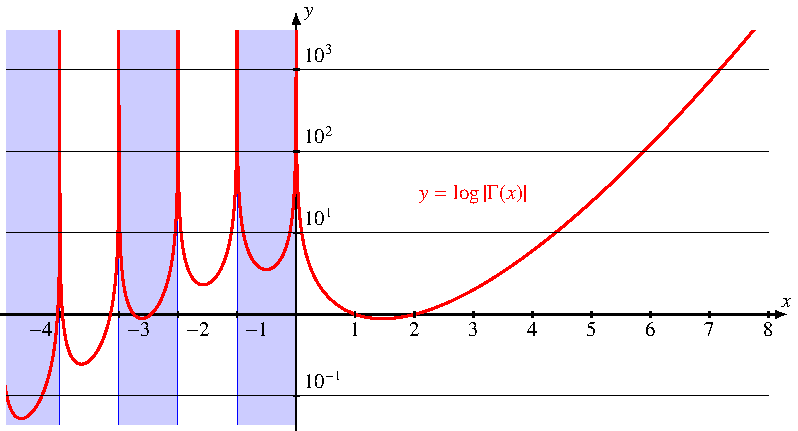
\includegraphics{chapters/040-rekursion/images/loggammaplot.pdf}
\caption{Der Graph der Funktion $\log|\Gamma(x)|$ ist für $x>0$ konvex. 
Die blau hinterlegten Bereiche zeigen an, wo die Gamma-Funktion
negative Werte annimmt.
\label{buch:rekursion:gamma:loggammaplot}}
\end{figure}
Die Integralformel und die Grenzwertdefinition für die Gamma-Funktion
zeigen beide, dass das Problem der Ausdehnung der Fakultät zu einer
Funktion $\mathbb{C}\to\mathbb{C}$ eine Lösung hat, aber es ist noch
nicht klar, in welchem Sinn dies die einzig mögliche Lösung ist.
Der Satz von Bohr-Mollerup gibt darauf eine Antwort.

Der Graph in Abbildung~\ref{buch:rekursion:gamma:loggammaplot}
zeigt, dass die Werte der Gamma-Funktion für $x>0$ so schnell
anwachsen, dass sogar die Funktion $\log|\Gamma(x)|$ konvex ist.
Der Satz von Bohr-Mollerup besagt, dass diese Eigenschaft zur
Charakterisierung der Gamma-Funktion verwendet werden kann.

\begin{satz}
\label{buch:satz:bohr-mollerup}
Eine Funktion $f\colon \mathbb{R}^+\to\mathbb{R}$ mit den Eigenschaften
\begin{enumerate}[i)]
\item $f(1)=1$,
\item $f(x+1)=xf(x)$ für alle $x\in\mathbb{R}^+$ und
\item die Funktion $\log f(t)$ ist konvex
\end{enumerate}
ist die Gamma-Funktion: $f(t)=\Gamma(t)$.
\index{Satz!von Bohr-Mollerup}%
\index{Bohr-Mollerup, Satz von}%
\end{satz}

Für den Beweis verwenden wir die folgende Eigenschaft einer konvexen
Funktion $g(x)$.
Sei
\begin{equation}
S(y,x) = \frac{g(y)-g(x)}{y-x}
\qquad\text{für $y-x$}
\end{equation}
die Steigung der Sekante zwischen den Punkten $(x,g(x))$ und $(y,g(y))$
des Graphen von $g$.
Da $g$ konvex ist, ist $S(y,x)$ eine monoton wachsende Funktion 
der beiden Variablen $x$ und $y$, solange $y>x$.

\begin{proof}[Beweis]
Wir halten zunächst fest, dass die Bedingungen i) und ii) zur Folge haben,
dass $f(n+1)=n!$ ist für alle positiven natürlichen Zahlen.
Für die Steigung einer Sekante der Funktion $g(x)=\log f(x)$ kann damit
für natürliche Argumente bereits berechnet werden, es ist
\[
S(n,n+1)
=
\frac{\log n! - \log (n-1)!}{n+1-n}
=
\frac{\log n + \log (n-1)! - \log(n-1)!}{1}
=
\log n
\]
und entsprechend auch $S(n-1,n) = \log(n-1)$.

\begin{figure}
\begin{center}
\begin{tikzpicture}[>=latex,thick]
\draw (-6,0) -- (6,0);

\node at (-5,0) [above] {$n-1\mathstrut$};
\node at (0,0) [above] {$n\mathstrut$};
\node at (3,0) [above] {$n+x\mathstrut$};
\node at (5,0) [above] {$n+1\mathstrut$};

\node[color=blue] at (-5,-2.3) {$S(n-1,n)\mathstrut$};
\node[color=red] at (-1.666,-2.3) {$S(n-1,n+x)\mathstrut$};
\node[color=darkgreen] at (1.666,-2.3) {$S(n,n+x)\mathstrut$};
\node[color=orange] at (5,-2.3) {$S(n,n+1)\mathstrut$};

\node at (-3.333,-2.3) {$<\mathstrut$};
\node at (0,-2.3) {$<\mathstrut$};
\node at (3.333,-2.3) {$<\mathstrut$};

\draw[color=blue] (-5,0) -- (-5,-2) -- (0,0);
\draw[color=red] (-5,0) -- (-1.666,-2) -- (3,0);
\draw[color=darkgreen] (0,0) -- (1.666,-2) -- (3,0);
\draw[color=orange] (0,0) -- (5,-2) -- (5,0);

\fill (-5,0) circle[radius=0.08];
\fill (0,0) circle[radius=0.08];
\fill (3,0) circle[radius=0.08];
\fill (5,0) circle[radius=0.08];

\draw[double,color=blue] (-5,-2.5) -- (-5,-3.0);
\draw[double,color=orange] (5,-2.5) -- (5,-3.0);

\node[color=blue] at (-5,-3.3) {$\log (n-1)\mathstrut$};
\node[color=orange] at (5,-3.3) {$\log (n)\mathstrut$};

\end{tikzpicture}
\end{center}
\caption{Für den Beweis des Satzes von Bohr-Mollerup wird die
Sekantensteigung $S(x,y)$ für die Argumente $n-1$, $n$, $n+x$ und $n+1$
verwendet.
\label{buch:rekursion:fig:bohr-mollerup}}
\end{figure}
Wir wenden jetzt die eben erwähnte Tatsache, dass $S(x,y)$ monoton
wachsend ist, auf die Punkte $n-1$, $n$, $n+x$ und $n+1$ wie
in Abbildung~\ref{buch:rekursion:fig:bohr-mollerup} an, wobei
$0<x<1$ ist.

Die linke Ungleichung in Abbildung~\ref{buch:rekursion:fig:bohr-mollerup}
ist
\begin{align}
\log(n-1)
&<
S(n-1,n+x)
=
\frac{\log f(n+x) -\log(n-2)!}{n+x-n+1}
\notag
\\
(x+1)\log(n-1) + \log(n-2)!
&< \log f(n+x),
\notag
\\
x\log(n-1) + \log(n-1)!
&< \log f(n+x)
\label{buch:rekursion:bohr-mollerup:eqn1}
\intertext{sie schätzt $\log f(n+x)$ nach unten ab.
Die Exponentialfunktion ist monoton wachsen, wendet man sie auf
\eqref{buch:rekursion:bohr-mollerup:eqn1} an, erhält man}
(n-1)^x (n-1)!
&<
f(n+x).
\label{buch:rekursion:bohr-mollerup:ungllinks}
\end{align}
Ganz ähnlich folgt aus der Ungleichung rechts in
Abbildung~\ref{buch:rekursion:fig:bohr-mollerup}
\begin{align}
\frac{\log f(n+x)-\log (n-1)!}{n+x-n}
&< \log n
\notag
\\
\log f(n+x) - \log(n-1)!
&<
x \log n
\notag
\\
\log f(n+x) 
&<
x\log n + \log(n-1)!
\notag
\intertext{und nach Anwendung der Exponentialfunktion}
f(n+x)
&<
n^x (n-1)!
\label{buch:rekursion:bohr-mollerup:unglrechts}
\end{align}
Die Funktion $f(n+x)$ können wir jetzt mit der Funktionalgleichung ii)
durch $f(x)$ ausdrücken:
\begin{align*}
f(n+x)
&=
(x+n-1)f(n+x-1)
\\
&=
(x+n-1)(x+n-2)f(n+x-2)
\\
&\vdots
\\
&=
(x+n-1)(x+n-2)\dots x\,f(x)
=
(x)_n f(x).
\end{align*}
Zusammen mit den Ungleichungen
\eqref{buch:rekursion:bohr-mollerup:ungllinks}
und
\eqref{buch:rekursion:bohr-mollerup:unglrechts}
erhalten wir
\begin{align*}
(n-1)^x (n-1)!
&<
(x)_n f(x)
<
n^x (n-1)!
\intertext{oder nach Division durch $(x)_n$}
%\underbrace{
\frac{(n-1)^x (n-1)!}{(x)_n}
%}_{\displaystyle\to \Gamma(x)}
&< f(x)
<
\frac{n^x (n-1)!}{(x)_n}
=
%\underbrace{
\frac{n^x n!}{(x)_{n+1}}
%}_{\displaystyle\to \Gamma(x)}
\cdot
%\underbrace{
\frac{x+n}{n}
%}_{\displaystyle\to 1}
.
\end{align*}
Der Ausdruck ganz links und der erste Bruch rechts konvergieren
für $n\to\infty$ beide gegen $\Gamma(x)$ und der Bruch ganz rechts
konvergiert gegen $1$.
Daher muss auch $f(x)=\Gamma(x)$ sein.
\end{proof}

%
% 12-integral.tex
%
% (c) 2022 Prof Dr Andreas Müller, OST Ostschweizer Hochschule
%
\subsection{Integraldarstellung und der Satz von Bohr-Mollerup
\label{buch:subsection:integral-eindeutig}}
Die Integralformel
\[
f(x)
=
\int_0^\infty t^{x-1}e^{-t}\,dt
\]
für die Gamma-Funktion erfüllt die Funktionalgleichung der Gamma-Funktion.
Aus dem Satz von Bohr-Mollerup~\ref{buch:satz:bohr-mollerup} folgt,
dass $f(x)=\Gamma(x)$, wenn gezeigt werden kann, dass $\log f(x)$
konvex ist.
Dies soll im Folgenden gezeigt werden.

\subsubsection{Logarithmische Ableitung}
\index{logarithmische Ableitung}%
Die Ableitungen der Funktion $\log f(x)$ sind die erste und
zweite logarithmische
\index{logarithmische Ableitung!zweite}%
Ableitung
\begin{align}
\frac{d}{dx}\log f(x)
&=
\frac{f'(x)}{f(x)}
\notag
\\
\frac{d^2}{dx^2} \log f(x)
&=
\frac{f''(x)f(x)-f'(x)^2}{f(x)^2}.
\label{buch:rekursion:eqn:zweiteablteitung}
\end{align}
Durch Ableiten unter dem Integralzeichen können die Ableitungen
von $f$ als
\begin{align*}
f'(x)
&=
\int_0^\infty \log(t)\, t^{x-1} e^{-t}\,dt
\\
f''(x)
&=
\int_0^\infty \log(t)^2\, t^{x-1} e^{-t}\,dt
\end{align*}
bestimmt werden.
Um nachzuweisen, dass $\log f(x)$ konvex ist, muss nur gezeigt werden,
dass die zweite logarithmische Ableitung von $f(x)$ positiv ist, was
gemäss~\eqref{buch:rekursion:eqn:zweiteablteitung} mit
\begin{equation}
f''(x)f(x)-f'(x)^2
=
\int_0^\infty \log(t)^2\, t^{x-1}e^{-t}\,dt
\int_0^\infty t^{x-1}e^{-t}\,dt
-
\biggl(
\int_0^\infty \log(t)\, t^{x-1}e^{-t}\,dt
\biggr)^2
\ge 0
\label{buch:rekursion:gamma-integral:ungleichung}
\end{equation}
gleichbedeutend ist.

\subsubsection{Skalarprodukt}
Die Integral in~\eqref{buch:rekursion:gamma-integral:ungleichung}
können als Werte eines Skalarproduktes von Funktionen auf $\mathbb{R}^+$
\index{Skalarprodukt}%
gelesen werden.
Dazu definieren wir
\begin{align}
\langle u,v\rangle
&=
\int_0^\infty u(t)v(t)\,t^{x-1}e^{-t}\,dt
\label{buch:rekursion:gamma-integral:eqn:skalarprodukt}
\\
\|u\|^2
&=
\int_0^\infty u(t)^2 \,t^{x-1}e^{-t}\,dt,
\notag
\end{align}
für alle Funktionen $u$ und $v$, für die die Integrale definiert sind.

\subsubsection{Cauchy-Schwarz-Ungleichung}
Die Cauchy-Schwarz-Ungleichung für das
Skalarprodukt~\eqref{buch:rekursion:gamma-integral:eqn:skalarprodukt}
\index{Cauchy-Schwarz-Ungleichung}
für die Funktion $u(t)=1$ und $v(t)=\log(t)$
lautet
\[
|\langle u,v\rangle|^2
=
\biggl|
\int_0^1 \log(t)\,t^{x-1}e^{-t}\,dt
\biggr|^2
\le
\|u\|^2\cdot \|v\|^2
=
\int_0^\infty 1\cdot t^{x-1}e^{-t}\,dt
\int_0^\infty \log(t)^2\cdot t^{x-1}e^{-t}\,dt.
\]
Daraus folgt aber durch Umstellen unmittelbar die
Ungleichung~\eqref{buch:rekursion:gamma-integral:ungleichung}.
Damit ist gezeigt, dass $\log f(t)$ konvex ist und nach
dem Satz~\ref{buch:satz:bohr-mollerup} folgt nun, dass $f(x)=\Gamma(x)$.



